% Self-contained tutorial. In Overleaf, upload this file as main.tex.
% Compiler: pdfLaTeX. No shell escape, external images, or .bib file required.
\documentclass[11pt,a4paper]{article}
\usepackage[T1]{fontenc}
\usepackage[utf8]{inputenc}
\usepackage{lmodern}
\usepackage[margin=23mm]{geometry}
\usepackage{microtype}
\DisableLigatures{encoding=T1,family=lmtt}
\usepackage{amsmath}
\usepackage{booktabs,tabularx,longtable,array}
\usepackage{xcolor}
\usepackage{listings}
\usepackage{enumitem}
\usepackage{graphicx}
\usepackage{tikz}
\usetikzlibrary{arrows.meta,positioning,fit,backgrounds}
\usepackage{needspace}
\usepackage{etoolbox}
\usepackage{xurl}
\usepackage{hyperref}
\hypersetup{colorlinks=true,linkcolor=black,citecolor=black,
  urlcolor=blue!50!black,pdftitle={Slurm and MPI on a Virtual Machine},
  pdfsubject={HPC software environment and workload management}}
\urlstyle{same}
\definecolor{codegray}{RGB}{247,247,247}
\definecolor{codeblue}{RGB}{24,57,94}
\lstdefinestyle{lab}{
  basicstyle=\ttfamily\small,columns=fullflexible,keepspaces=true,
  showstringspaces=false,breaklines=true,breakatwhitespace=false,
  postbreak=\mbox{\textcolor{gray}{$\hookrightarrow$}\space},
  backgroundcolor=\color{codegray},frame=single,
  rulecolor=\color{black!15},framerule=0.3pt,
  xleftmargin=5pt,xrightmargin=5pt,framexleftmargin=4pt,
  framexrightmargin=4pt,aboveskip=9pt,belowskip=9pt,
  keywordstyle=\color{codeblue},commentstyle=\color{black!65},
  stringstyle=\color{black},upquote=true,tabsize=4}
\lstset{style=lab}
\setlist[itemize]{leftmargin=1.5em,itemsep=3pt,topsep=5pt}
\setlist[enumerate]{leftmargin=1.7em,itemsep=4pt,topsep=5pt}
\setlength{\parindent}{0pt}
\setlength{\parskip}{6pt}
\setlength{\emergencystretch}{2em}
\renewcommand{\arraystretch}{1.2}
\newcolumntype{Y}{>{\raggedright\arraybackslash}X}
\newcolumntype{P}[1]{>{\raggedright\arraybackslash}p{#1}}
\newcommand{\checkpoint}[1]{\par\textbf{Checkpoint.} #1\par}
\newcommand{\task}[1]{\par\textbf{Try it.} #1\par}
\newcommand{\cmd}[1]{\texttt{\detokenize{#1}}}
\pretocmd{\section}{\Needspace{9\baselineskip}}{}{}
\pretocmd{\subsection}{\Needspace{7\baselineskip}}{}{}
\title{\textbf{Slurm and MPI on a Virtual Machine}\\[5pt]
  \large HPC Software Environment and Workload Management}
\author{Practical laboratory tutorial}
\date{Reference platform: Ubuntu Server 24.04 LTS\\September 2026}
\begin{document}
\maketitle

This tutorial turns one PC or laptop into a small HPC learning environment.
You will create one Linux virtual machine (VM), install a compiler and an MPI
implementation, configure Slurm, and submit parallel applications through a
job queue. The same VM acts as the submission host, Slurm controller, and
compute node. No second computer or cloud account is required.

The central relationship is simple: \textbf{Slurm decides when and where a job
can run and allocates its resources; MPI lets the processes in a parallel
program exchange data and coordinate their work.} Installing Slurm does not
automatically parallelize a sequential program.

\section*{Learning outcomes}
After completing the laboratory, you should be able to:
\begin{enumerate}
\item Identify the components of an HPC software environment: Linux, shell,
      filesystems, compilers, libraries, MPI, environment configuration, and
      a workload manager.
\item Configure a small Slurm environment and explain the roles of the
      controller, compute daemon, authentication service, and partition.
\item Request resources, submit and monitor jobs, inspect logs, cancel jobs,
      and diagnose common pending and failure states.
\item Compile and launch MPI applications inside Slurm allocations and
      distinguish nodes, tasks, ranks, CPUs, and threads.
\item Measure MPI execution time and discuss speedup without confusing
      queue waiting time with computation time.
\end{enumerate}

\textbf{Suggested pacing.} Allow one preparation session for the VM and
software setup, followed by two laboratory sessions of roughly two hours:
first job management, then MPI and experiments. Download and installation
time depend on your connection and machine.

\textbf{Prerequisites.} Basic Linux commands, a text editor, elementary C,
and an introductory understanding of MPI ranks and collective operations.
All commands are executed in the Ubuntu guest, except when configuring the
VM in the host's virtualization application.

\clearpage
\tableofcontents
\clearpage

\section{Plan the virtual laboratory}
\subsection{Hardware and operating system}
Use a fresh Ubuntu Server 24.04 LTS VM with a normal user account that can run
\cmd{sudo}. Ubuntu Desktop 24.04 can also be used, but its graphical desktop
leaves fewer resources for jobs. The Ubuntu repositories provide Slurm
23.11.x and Open MPI 4.1.x for this release; record the actual package versions
installed on your machine.\cite{ubuntu-slurm,ubuntu-mpi}

\begin{tabularx}{\linewidth}{@{}P{0.25\linewidth}YY@{}}
\toprule
Resource & Minimum laboratory setup & More comfortable setup \\
\midrule
Host memory & 8 GiB with other applications closed & 16 GiB or more \\
VM virtual CPUs & 2 vCPUs & 4 vCPUs \\
VM memory & 4 GiB & 4--6 GiB \\
VM virtual disk & 25 GiB, dynamically allocated & 30 GiB or more \\
VM network & NAT with internet access for installation & Same \\
\bottomrule
\end{tabularx}

A vCPU is a processor presented to the guest by the hypervisor. It is not
necessarily a dedicated physical core. Do not assign all host memory to the
guest or increase vCPU counts beyond what your host can use effectively.

\begin{enumerate}
\item Create a VM in a virtualization application supported by your host,
      such as VirtualBox or VMware. Use a guest image matching the host
      architecture; an ARM host needs an appropriate ARM guest/hypervisor.
\item Attach the Ubuntu Server installation ISO and install Ubuntu onto the
      \emph{virtual disk}. The official installation guide explains the
      installer screens.\cite{ubuntu-install}
\item Create a regular user, for example \cmd{student}. A hostname such as
      \cmd{hpcvm} is convenient, but the configuration script detects yours.
\item Boot into Ubuntu, log in, and open its terminal. NAT networking is
      sufficient. SSH and a bridged network are not needed for this lab.
\item Take a VM snapshot before changing the Slurm configuration.
\end{enumerate}

The main instructions require only two vCPUs. Four-rank experiments are
optional and should be skipped if Slurm reports fewer than four CPUs.

\subsection{What this laboratory represents}
MPI uses separate processes with separate address spaces, including when all
ranks run on one VM. Open MPI can communicate between local ranks using a
shared-memory transport. This is real MPI execution, but it does not measure
communication across physical computers or an HPC interconnect.

Slurm services, operating-system activity, and MPI ranks share the same VM.
The configuration is suitable for learning on a private VM. It deliberately
omits a database service and cgroup resource containment. Memory requests
guide scheduling, but this setup does not enforce them as hard memory limits.

\section{Understand the HPC software environment}
\subsection{The components and their roles}
\begin{tabularx}{\linewidth}{@{}P{0.23\linewidth}P{0.24\linewidth}Y@{}}
\toprule
Layer & Tool used here & Purpose \\
\midrule
Guest operating system & Ubuntu Linux & Processes, virtual memory, files, networking, and user accounts \\
Shell and build tools & Bash, Make, GCC & Edit source files, run commands, compile, and organize builds \\
MPI implementation & Open MPI & MPI library and runtime for cooperating parallel processes \\
Environment configuration & Environment Modules & Set and restore software-related shell variables \\
Workload manager & Slurm & Allocate resources and schedule and manage jobs \\
Authentication & MUNGE & Create and validate credentials used by Slurm \\
Application & C programs in this tutorial & Perform the actual computation \\
\bottomrule
\end{tabularx}

\cmd{mpicc} is a compiler wrapper. It invokes a C compiler with the include
paths and libraries needed for MPI. \cmd{mpirun} launches MPI processes.
\cmd{sbatch} submits a job to Slurm; it does not compile your source code.
MUNGE authentication is separate from the application's MPI communication.
\cite{slurm-overview,munge}

\subsection{How the services work together}
\begin{center}
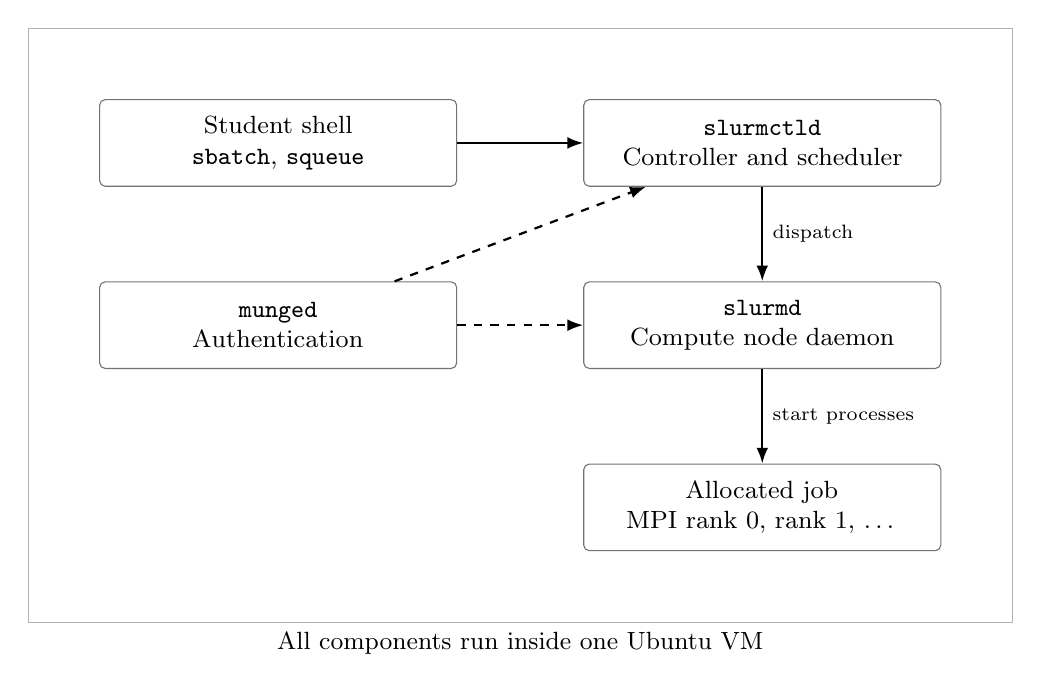
\begin{tikzpicture}[
  node distance=12mm and 16mm,
  box/.style={draw=black!55,rounded corners=2pt,align=center,
    minimum height=11mm,text width=43mm,font=\small},
  arr/.style={-{Latex[length=2mm]},thick}]
\node[box] (cli) {Student shell\\\cmd{sbatch}, \cmd{squeue}};
\node[box,right=of cli] (ctl) {\cmd{slurmctld}\\Controller and scheduler};
\node[box,below=of ctl] (daemon) {\cmd{slurmd}\\Compute node daemon};
\node[box,left=of daemon] (auth) {\cmd{munged}\\Authentication};
\node[box,below=of daemon] (job) {Allocated job\\MPI rank 0, rank 1, \ldots};
\draw[arr] (cli) -- (ctl);
\draw[arr] (ctl) -- node[right,font=\scriptsize]{dispatch} (daemon);
\draw[arr] (daemon) -- node[right,font=\scriptsize]{start processes} (job);
\draw[arr,dashed] (auth) -- (ctl);
\draw[arr,dashed] (auth) -- (daemon);
\begin{scope}[on background layer]
\node[draw=black!30,inner sep=9mm,fit=(cli)(ctl)(auth)(job),
  label={[font=\small]below:All components run inside one Ubuntu VM}] {};
\end{scope}
\end{tikzpicture}
\end{center}
The controller maintains cluster and job state. The compute daemon launches
work on its node; Slurm uses \cmd{slurmstepd} processes to manage job steps.
A \emph{partition} is a named collection of nodes with scheduling limits and
access rules. This lab has one partition, \cmd{debug}, containing one node.
\cite{slurm-admin,slurm-overview}

\subsection{Vocabulary before commands}
\begin{description}[style=nextline,leftmargin=0pt,labelwidth=0pt,labelsep=0pt]
\item[Job] A request to run work under Slurm, identified by a job ID.
\item[Allocation] The resources assigned to the job for a period of time.
\item[Job step] An execution within an allocation, commonly started with
\cmd{srun}. One job can contain several steps.
\item[Node] A compute machine known to Slurm. Our VM is one node.
\item[Task] A process requested or launched by Slurm. In these MPI examples,
one requested task corresponds to one MPI rank.
\item[Rank] A process identifier within an MPI communicator. Ranks in
\cmd{MPI_COMM_WORLD} are numbered from zero.
\item[CPU per task] A CPU allocation for each task. Depending on site
configuration, a Slurm CPU can represent a core or hardware thread.
\end{description}

For a pure MPI job, request one CPU per task. For a program with two MPI
ranks, each running two OpenMP threads, request two tasks and two CPUs per
task, and configure two threads in the application. Allocating more CPUs
does not cause a single-threaded program to use them automatically.

\section{Install and inspect the software}
\subsection{Install the Ubuntu packages}
Run the following inside the VM. Use \cmd{sudo} for installation and service
administration; later compile and submit jobs as your regular user.
\par\nobreak
\begin{minipage}{\linewidth}
\begin{lstlisting}[language=bash]
sudo apt update
sudo apt install -y software-properties-common
sudo add-apt-repository -y universe
sudo apt update
sudo apt install -y build-essential openmpi-bin libopenmpi-dev \
  munge slurmctld slurmd slurm-client slurm-wlm-basic-plugins \
  environment-modules python3 unzip nano
\end{lstlisting}
\end{minipage}\par

The Slurm packages may attempt to start services before a configuration
exists. If they report a missing \cmd{slurm.conf}, finish the configuration
below and start the services afterward. Do not substitute the unrelated
package named \cmd{slurm}, which is a network-monitoring utility.

Inspect the guest and installed tools:
\par\nobreak
\begin{minipage}{\linewidth}
\begin{lstlisting}[language=bash]
hostname -s
lscpu
free -h
df -h "$HOME"
gcc --version
mpicc --showme:command
mpicc --showme:link
mpirun --version
sinfo --version
dpkg-query -W slurmctld slurmd openmpi-bin libopenmpi-dev
\end{lstlisting}
\end{minipage}\par

\checkpoint{Record the hostname, vCPU count, memory, Slurm version, and
Open MPI version. The version command works before the Slurm controller
starts; a normal \cmd{sinfo} query will require the controller.}

\subsection{Start and check MUNGE}
Ubuntu normally creates a MUNGE key during package installation.
\par\nobreak
\begin{minipage}{\linewidth}
\begin{lstlisting}[language=bash]
sudo test -s /etc/munge/munge.key
sudo systemctl enable --now munge
munge -n | unmunge
\end{lstlisting}
\end{minipage}\par

The decoded credential should include \cmd{STATUS: Success (0)}. Do not
continue if this fails. Check \cmd{sudo journalctl -u munge -n 40 --no-pager}.
Troubleshooting instructions for a missing key appear later.

\subsection{Prepare the working directory}
The companion archive contains a top-level folder named \cmd{slurm-lab}.
Copy the archive into the VM, then extract it into your home directory. The
example below assumes that the archive is in your current directory.
\par\nobreak
\begin{minipage}{\linewidth}
\begin{lstlisting}[language=bash]
unzip Slurm_MPI_VM_Lab_Files.zip -d "$HOME"
cd "$HOME/slurm-lab"
mkdir -p jobs logs results
\end{lstlisting}
\end{minipage}\par

If working only from this document, create \cmd{~/slurm-lab} and its
\cmd{jobs}, \cmd{logs}, and \cmd{results} subdirectories, then create the
files from the listings with \cmd{nano}. The core lab does not depend on
downloading code from another website.

\textbf{Command convention.} Shell blocks contain commands without a prompt
symbol. A block introduced as a filename is the \emph{content of that file}.
Save it with Unix line endings. For long listings, a printed continuation
arrow indicates visual wrapping, not an extra character to type. The
companion files avoid copying code from a PDF.

\section{Configure a single Slurm node}
\subsection{Detect the VM resources}
\par\nobreak
\begin{minipage}{\linewidth}
\begin{lstlisting}[language=bash]
sudo systemctl stop slurmd slurmctld
/usr/sbin/slurmd -C
\end{lstlisting}
\end{minipage}\par

\cmd{slurmd -C} prints the hardware description Slurm detects. The script
below keeps that CPU topology and advertises 80\% of detected memory to
Slurm, leaving scheduling headroom for Linux and the services. This memory
reservation is a scheduling convention, not an operating-system memory
barrier.

\subsection{Create the configuration script}
Save the following two consecutive listings in one file named
\cmd{configure_single_vm.sh}. The file is already present in the companion
archive. It refuses to overwrite an existing \cmd{/etc/slurm/slurm.conf}.
It is intended for the fresh VM created in this tutorial.
\begin{lstlisting}[language=bash]
#!/usr/bin/env bash
# Run with sudo, once, after installing the Ubuntu packages.
set -euo pipefail
if (( EUID != 0 )); then
    echo "Run: sudo bash configure_single_vm.sh" >&2
    exit 1
fi
if [[ -e /etc/slurm/slurm.conf ]]; then
    echo "Existing slurm.conf found; leaving it unchanged." >&2
    exit 1
fi
lab_node=$(hostname -s)
lab_detected=$(/usr/sbin/slurmd -C | awk '/^NodeName=/{print; exit}')
if [[ ! "$lab_detected" =~ RealMemory=([0-9]+) ]]; then
    echo "Cannot detect node memory." >&2
    exit 1
fi
lab_memory=$(( BASH_REMATCH[1] * 80 / 100 ))
if (( lab_memory < 1536 )); then
    echo "Assign at least 4 GiB RAM to the VM, then retry." >&2
    exit 1
fi
lab_node_line=$(printf '%s\n' "$lab_detected" |
    sed -E "s/RealMemory=[0-9]+/RealMemory=${lab_memory}/")
install -d -m 0755 /etc/slurm
install -d -o slurm -g slurm -m 0755 /var/spool/slurmctld
install -d -o root -g root -m 0755 /var/spool/slurmd
install -d -o slurm -g slurm -m 0755 /var/log/slurm
\end{lstlisting}

Continue in the \emph{same file} with the following lines. Keep the final
\cmd{EOF} at the start of its line.
\begin{lstlisting}[language=bash]
cat > /etc/slurm/slurm.conf <<EOF
ClusterName=laptoplab
SlurmctldHost=${lab_node}(127.0.0.1)
SlurmUser=slurm
SlurmdUser=root
AuthType=auth/munge
CredType=cred/munge
StateSaveLocation=/var/spool/slurmctld
SlurmdSpoolDir=/var/spool/slurmd
SlurmctldPidFile=/run/slurmctld.pid
SlurmdPidFile=/run/slurmd.pid
SlurmctldLogFile=/var/log/slurm/slurmctld.log
SlurmdLogFile=/var/log/slurm/slurmd.log
SchedulerType=sched/backfill
SelectType=select/cons_tres
SelectTypeParameters=CR_CPU_Memory
TaskPlugin=task/affinity
ProctrackType=proctrack/pgid
ReturnToService=1
AccountingStorageType=accounting_storage/none
JobAcctGatherType=jobacct_gather/linux
JobCompType=jobcomp/filetxt
JobCompLoc=/var/log/slurm/jobcomp.log
MinJobAge=86400
DefMemPerCPU=256
${lab_node_line} NodeAddr=127.0.0.1 State=UNKNOWN
PartitionName=debug Nodes=${lab_node} Default=YES MaxTime=01:00:00 State=UP OverSubscribe=NO
EOF
chmod 0644 /etc/slurm/slurm.conf
echo "Created /etc/slurm/slurm.conf for ${lab_node}."
echo "Read the file before starting the Slurm services."
\end{lstlisting}

\cmd{127.0.0.1} refers to this VM. Both daemons can therefore contact each
other without relying on external name resolution. These loopback addresses
are only suitable for this single-VM arrangement.

\subsection{Apply the configuration and start Slurm}
\par\nobreak
\begin{minipage}{\linewidth}
\begin{lstlisting}[language=bash]
cd "$HOME/slurm-lab"
sudo bash configure_single_vm.sh
cat /etc/slurm/slurm.conf
sudo systemctl enable --now slurmctld
sudo systemctl enable --now slurmd
systemctl is-active munge slurmctld slurmd
scontrol ping
sinfo -N -l
scontrol show node "$(hostname -s)"
srun --partition=debug --nodes=1 --ntasks=1 \
  --mem=256M --time=00:01:00 hostname
\end{lstlisting}
\end{minipage}\par

\checkpoint{All three services report \cmd{active}; the controller reports
\cmd{UP}; the node becomes \cmd{idle}; and the \cmd{srun} command prints the
VM's hostname. Initial node registration can take a few seconds. If the node
is down or drained, inspect its reason before continuing.}

\subsection{Read the important configuration choices}
\begin{tabularx}{\linewidth}{@{}P{0.40\linewidth}Y@{}}
\toprule
Setting & Consequence in this lab \\
\midrule
\cmd{select/cons_tres} and \cmd{CR_CPU_Memory} & Schedule CPU and memory as consumable resources. \\
\cmd{OverSubscribe=NO} & Do not allocate the same CPU to multiple jobs at once; jobs may still share a node if different CPUs are available. \\
\cmd{task/affinity} & Bind tasks to CPUs; this is not cgroup containment. \\
\cmd{proctrack/pgid} & Track process groups for this simple teaching setup. \\
\cmd{jobcomp/filetxt} & Write completed-job summaries to a text log. \\
\cmd{MinJobAge=86400} & Keep completed jobs in controller memory for at least a day before normal age-based purging. \\
\cmd{accounting_storage/none} & Omit the accounting database; ordinary \cmd{sacct} history is not configured. \\
\bottomrule
\end{tabularx}

Production installations commonly use cgroups for stronger process tracking
and enforcement and a database for accounting. The local \cmd{man slurm.conf}
documents the options for your installed release.\cite{slurm-conf}

\section{Inspect and control the software environment}
\subsection{Paths and compiler consistency}
\par\nobreak
\begin{minipage}{\linewidth}
\begin{lstlisting}[language=bash]
command -v gcc mpicc mpirun sbatch srun
printf '%s\n' "$PATH"
mpicc --showme
ompi_info | grep -i slurm
\end{lstlisting}
\end{minipage}\par

Compile and launch with the same MPI implementation. A binary built with one
MPI library should not be assumed compatible with a launcher from a different
installation. The distribution's Open MPI tools provide one consistent
toolchain for this lab.

\subsection{A small Environment Modules exercise}
HPC sites often install several compiler and MPI versions. Modules modify
the shell environment so a chosen installation can be found. A module does
not install a package or create a Slurm allocation.\cite{modules}

This VM uses system packages, so do not assume a module named
\cmd{openmpi} already exists. Create a small local module instead:
\par\nobreak
\begin{minipage}{\linewidth}
\begin{lstlisting}[language=bash]
mkdir -p "$HOME/modulefiles/lab"
cat > "$HOME/modulefiles/lab/1.0" <<'EOF'
#%Module1.0
module-whatis "Environment for the Slurm and MPI lab"
setenv HPC_LAB_ROOT $env(HOME)/slurm-lab
setenv OMP_NUM_THREADS 1
EOF
source /etc/profile.d/modules.sh
module use "$HOME/modulefiles"
module avail
module load lab/1.0
module list
printf '%s\n' "$HPC_LAB_ROOT" "$OMP_NUM_THREADS"
module unload lab/1.0
\end{lstlisting}
\end{minipage}\par

The module intentionally configures the lab variables, rather than claiming
to switch between multiple MPI installations. Real compiler/MPI modules
usually also alter paths to select their own binaries and libraries.

If a batch script needs a module, initialize and load it \emph{inside} the
script, after the \texttt{\#SBATCH} directives. A batch shell need not read the
same startup files as an interactive shell. The provided MPI scripts use
system paths and explicitly set their thread count, so this example module
is not required by them.

\task{Explain the difference between installing a software package, loading
a module, compiling an executable, and submitting a job.}

\section{Submit and inspect the first batch job}
\subsection{Write the script}
Save this file as \cmd{jobs/hello.sbatch}:
\par\nobreak
\begin{minipage}{\linewidth}
\begin{lstlisting}[language=bash]
#!/usr/bin/env bash
#SBATCH --job-name=hello
#SBATCH --partition=debug
#SBATCH --nodes=1
#SBATCH --ntasks=1
#SBATCH --cpus-per-task=1
#SBATCH --mem=256M
#SBATCH --time=00:02:00
#SBATCH --output=logs/hello-%j.out
#SBATCH --error=logs/hello-%j.err
set -euo pipefail
cd "$SLURM_SUBMIT_DIR"
echo "Job: $SLURM_JOB_ID"
echo "Nodes: $SLURM_JOB_NODELIST"
echo "Working directory: $PWD"
date -Is
srun --ntasks=1 hostname
srun --ntasks=1 sleep 15
date -Is
\end{lstlisting}
\end{minipage}\par


\texttt{\#SBATCH} lines are read by Slurm. Keep them before the first executable
statement. Shell variables are not expanded in these directives: for
example, \texttt{\#SBATCH --output=\$HOME/result.out} is not a reliable way to
choose the home directory. Here, paths are relative to the submission
directory, and \texttt{\%j} is replaced with the job ID.\cite{slurm-sbatch}

The output directory must exist \emph{before submission}. Slurm opens log
files before the script executes; putting only \cmd{mkdir -p logs} inside
the script is too late. \cmd{set -euo pipefail} helps this script report
command failures instead of silently continuing.

\subsection{Submit as the regular user}
\par\nobreak
\begin{minipage}{\linewidth}
\begin{lstlisting}[language=bash]
cd "$HOME/slurm-lab"
mkdir -p logs
jobid=$(sbatch --parsable jobs/hello.sbatch)
echo "Submitted job $jobid"
squeue -u "$USER"
scontrol show job "$jobid"
\end{lstlisting}
\end{minipage}\par

\cmd{sbatch} returns once the controller accepts the job. That does not mean
the job has finished, or even started. Wait for it to leave the queue, then
read the results:
\par\nobreak
\begin{minipage}{\linewidth}
\begin{lstlisting}[language=bash]
cat "logs/hello-${jobid}.out"
cat "logs/hello-${jobid}.err"
scontrol show job "$jobid"
\end{lstlisting}
\end{minipage}\par

\checkpoint{The output contains the job ID, VM hostname, and timestamps.
After completion, the controller record should show \cmd{COMPLETED} and
\cmd{ExitCode=0:0}. An empty error file is normal.}

\textbf{Submission method matters.} \cmd{sbatch jobs/hello.sbatch} submits
the script to Slurm. \cmd{bash jobs/hello.sbatch} treats the directives as
comments and runs outside a new Slurm allocation. The latter will also fail
on unset Slurm variables in these examples.

\subsection{Interpret the resource request}
\begin{tabularx}{\linewidth}{@{}P{0.30\linewidth}Y@{}}
\toprule
Option & Meaning \\
\midrule
\cmd{--nodes=1} & Use one compute node. \\
\cmd{--ntasks=2} & Request two tasks; our MPI scripts launch two ranks. \\
\cmd{--cpus-per-task=1} & Allocate one CPU per task. \\
\cmd{--mem=512M} & Request 512 MiB per node, not per rank. \\
\cmd{--mem-per-cpu=256M} & Alternative request of 256 MiB per allocated CPU; do not combine it with \cmd{--mem}. \\
\cmd{--time=00:02:00} & Set a two-minute running-time limit; waiting in the queue does not consume it. \\
\bottomrule
\end{tabularx}

For the pure MPI examples, requested task CPUs are
\(\text{tasks}\times\text{CPUs per task}\). Node topology and options such as
\cmd{--exclusive} can make the overall allocation larger.

\section{Use allocations and job steps interactively}
\cmd{salloc} obtains an allocation and starts a shell on the submission host
by default. Use \cmd{srun} to execute work on the allocated node. The two
hosts happen to be the same VM here, so the distinction is less visible.
\cite{slurm-salloc,slurm-srun}

\par\nobreak
\begin{minipage}{\linewidth}
\begin{lstlisting}[language=bash]
salloc --partition=debug --nodes=1 --ntasks=2 \
  --cpus-per-task=1 --mem=512M --time=00:05:00
# Continue after the allocation has been granted.
echo "$SLURM_JOB_ID"
srun --ntasks=2 --label hostname
srun --ntasks=2 --label bash -c \
  'echo "task=$SLURM_PROCID local=$SLURM_LOCALID host=$(hostname)"'
srun --ntasks=1 date -Is
exit
\end{lstlisting}
\end{minipage}\par

Type \cmd{exit} once to leave the allocation shell and release resources.
Do not leave an unused interactive allocation running while trying the
batch-job exercises.

The first two \cmd{srun} commands launch two separate processes. Seeing the
same hostname twice is expected. These programs are ordinary Linux commands,
not MPI programs; launching several commands does not give them MPI
communication logic.

\begin{tabularx}{\linewidth}{@{}P{0.20\linewidth}YY@{}}
\toprule
Command & Primary action & Typical use \\
\midrule
\cmd{sbatch} & Submit a script; usually return immediately & Reproducible unattended runs \\
\cmd{salloc} & Reserve resources and provide a shell context & Interactive development \\
\cmd{srun} & Launch a step; can obtain an allocation when used outside one & Execute processes on allocated resources \\
\cmd{mpirun} & Launch cooperating MPI ranks & MPI runtime inside a Slurm allocation \\
\bottomrule
\end{tabularx}

\task{Why does \cmd{--ntasks=2} differ from
\cmd{--ntasks=1 --cpus-per-task=2}? Which one matches two single-threaded
MPI ranks?}

\clearpage
\section{Observe scheduling and manage job states}
\subsection{Create visible resource contention}
Save \cmd{jobs/hold_node.sbatch}:
\par\nobreak
\begin{minipage}{\linewidth}
\begin{lstlisting}[language=bash]
#!/usr/bin/env bash
#SBATCH --job-name=hold-node
#SBATCH --partition=debug
#SBATCH --nodes=1
#SBATCH --ntasks=1
#SBATCH --cpus-per-task=1
#SBATCH --exclusive
#SBATCH --mem=512M
#SBATCH --time=00:04:00
#SBATCH --output=logs/hold-%j.out
set -euo pipefail
echo "Holding the node for 180 seconds"
srun --ntasks=1 sleep 180
\end{lstlisting}
\end{minipage}\par


This job reserves the whole node using \cmd{--exclusive}, even though its
single task mostly sleeps. Allocation and actual CPU utilization are
different quantities.\cite{slurm-sbatch}

\par\nobreak
\begin{minipage}{\linewidth}
\begin{lstlisting}[language=bash]
cd "$HOME/slurm-lab"
blocker=$(sbatch --parsable jobs/hold_node.sbatch)
squeue -j "$blocker"
\end{lstlisting}
\end{minipage}\par

Wait until the blocker is \cmd{RUNNING} (\cmd{R}), then submit another job:
\par\nobreak
\begin{minipage}{\linewidth}
\begin{lstlisting}[language=bash]
waiting=$(sbatch --parsable jobs/hello.sbatch)
squeue -u "$USER" -o "%.10i %.14j %.10T %.10M %.20R"
scontrol show job "$waiting"
\end{lstlisting}
\end{minipage}\par

The second job should remain \cmd{PENDING} while the node is occupied. Its
reason will commonly be \cmd{Resources}; transient scheduling reasons can
differ. Take a screenshot showing both jobs, then release the node:
\par\nobreak
\begin{minipage}{\linewidth}
\begin{lstlisting}[language=bash]
scancel "$blocker"
squeue -u "$USER"
scontrol show job "$blocker"
\end{lstlisting}
\end{minipage}\par

\checkpoint{The blocker becomes \cmd{CANCELLED}, and the waiting job can
start after Slurm finishes cleaning up the cancelled job.}

\cmd{scancel} targets a job by its ID. Cancel only your intended experiment.
An empty \cmd{squeue} means no matching active or pending jobs; it does not
prove that a finished job succeeded.\cite{slurm-squeue,slurm-scancel}

\subsection{Distinguish pending and terminal states}
\begin{tabularx}{\linewidth}{@{}P{0.27\linewidth}Y@{}}
\toprule
State & Interpretation \\
\midrule
\cmd{PENDING} / \cmd{PD} & Waiting for resources, eligibility, a dependency, or another scheduling condition \\
\cmd{RUNNING} / \cmd{R} & Has begun executing in an allocation \\
\cmd{COMPLETING} / \cmd{CG} & Execution ended; cleanup is still in progress \\
\cmd{COMPLETED} / \cmd{CD} & Finished successfully as reported to Slurm \\
\cmd{FAILED} / \cmd{F} & Failed, for example because the batch script returned a nonzero status \\
\cmd{CANCELLED} / \cmd{CA} & Cancelled by a user or administrator \\
\cmd{TIMEOUT} / \cmd{TO} & Exceeded the configured running-time limit \\
\bottomrule
\end{tabularx}
These are common states; Slurm defines additional states and flags.
Always inspect the reason and logs. A completed state also does not prove
that your numerical answer is correct.\cite{slurm-states}

\subsection{Generate a controlled failure and timeout}
\par\nobreak
\begin{minipage}{\linewidth}
\begin{lstlisting}[language=bash]
failed=$(sbatch --parsable --job-name=exit7 --partition=debug \
  --ntasks=1 --mem=256M --time=00:01:00 \
  --output=logs/exit7-%j.out --wrap='exit 7')
timed=$(sbatch --parsable --job-name=timeout --partition=debug \
  --ntasks=1 --mem=256M --time=00:01:00 \
  --output=logs/timeout-%j.out --wrap='srun sleep 180')
squeue -u "$USER"
\end{lstlisting}
\end{minipage}\par

After the jobs finish, inspect them. Time-limit termination is subject to
Slurm's polling and cleanup; it is not a precise stopwatch event.
\par\nobreak
\begin{minipage}{\linewidth}
\begin{lstlisting}[language=bash]
scontrol show job "$failed"
scontrol show job "$timed"
sudo tail -n 10 /var/log/slurm/jobcomp.log
\end{lstlisting}
\end{minipage}\par

Expect \cmd{FAILED} with \cmd{ExitCode=7:0} for the first job and
\cmd{TIMEOUT} for the second. The colon separates the exit status from the
terminating signal in the job record.

\subsection{Historical records without a database}
This lab retains recent controller records and writes a completion log.
It does not configure \cmd{slurmdbd}, so ordinary \cmd{sacct} database
queries are not a required checkpoint. On a production cluster with
accounting enabled, a useful query is:
\par\nobreak
\begin{minipage}{\linewidth}
\begin{lstlisting}[language=bash]
# Production cluster example; requires configured accounting.
sacct -j JOBID --format=JobID,JobName,State,Elapsed,AllocCPUS,ExitCode
\end{lstlisting}
\end{minipage}\par

Recent \cmd{scontrol} records are temporary. Preserve job scripts, output
files, version information, and measurements for your report.
\cite{slurm-sacct,slurm-scontrol}

\section{Run an MPI program through Slurm}
\subsection{Write and compile a program that proves cooperation}
Save the following as \cmd{mpi_hello.c}:
\par\nobreak
\begin{minipage}{\linewidth}
\begin{lstlisting}[language=C]
#include <mpi.h>
#include <stdio.h>

int main(int argc, char **argv) {
    int rank, size, length, rank_sum;
    char node[MPI_MAX_PROCESSOR_NAME];
    MPI_Init(&argc, &argv);
    MPI_Comm_rank(MPI_COMM_WORLD, &rank);
    MPI_Comm_size(MPI_COMM_WORLD, &size);
    MPI_Get_processor_name(node, &length);
    printf("Hello from rank %d of %d on %s\n", rank, size, node);
    MPI_Reduce(&rank, &rank_sum, 1, MPI_INT, MPI_SUM,
               0, MPI_COMM_WORLD);
    if (rank == 0) {
        printf("CHECK ranks=%d sum=%d expected=%d\n",
               size, rank_sum, size * (size - 1) / 2);
    }
    MPI_Finalize();
    return 0;
}
\end{lstlisting}
\end{minipage}\par


The program prints each rank's identity and uses \cmd{MPI_Reduce} to add all
rank numbers at rank 0. With two ranks the expected sum is 1; with four it
is 6. This checks more than simply printing the hostname twice.
\par\nobreak
\begin{minipage}{\linewidth}
\begin{lstlisting}[language=bash]
cd "$HOME/slurm-lab"
mpicc -O2 -Wall -Wextra -std=c11 mpi_hello.c -o mpi_hello
\end{lstlisting}
\end{minipage}\par


\subsection{Submit the MPI job}
Save \cmd{jobs/mpi_hello.sbatch}:
\par\nobreak
\begin{minipage}{\linewidth}
\begin{lstlisting}[language=bash]
#!/usr/bin/env bash
#SBATCH --job-name=mpi-hello
#SBATCH --partition=debug
#SBATCH --nodes=1
#SBATCH --ntasks=2
#SBATCH --cpus-per-task=1
#SBATCH --mem=512M
#SBATCH --time=00:02:00
#SBATCH --output=logs/mpi-hello-%j.out
#SBATCH --error=logs/mpi-hello-%j.err
set -euo pipefail
cd "$SLURM_SUBMIT_DIR"
export OMP_NUM_THREADS=1
mpirun -np "$SLURM_NTASKS" ./mpi_hello
\end{lstlisting}
\end{minipage}\par

\par\nobreak
\begin{minipage}{\linewidth}
\begin{lstlisting}[language=bash]
mpi_job=$(sbatch --wait --parsable jobs/mpi_hello.sbatch)
cat "logs/mpi-hello-${mpi_job}.out"
cat "logs/mpi-hello-${mpi_job}.err"
\end{lstlisting}
\end{minipage}\par

Here, \cmd{--wait} makes the submission command wait until termination.
Its return status reflects the job's result. If it fails, inspect both log
files and the controller record.

Expected content, with the rank lines possibly in a different order:
\par\nobreak
\begin{minipage}{\linewidth}
\begin{lstlisting}
Hello from rank 0 of 2 on hpcvm
Hello from rank 1 of 2 on hpcvm
CHECK ranks=2 sum=1 expected=1
\end{lstlisting}
\end{minipage}\par

Your hostname may differ. Output ordering depends on execution and buffering;
do not treat a different order as an error.

Slurm runs \emph{one copy of the batch script}. The request
\cmd{--ntasks=2} does not cause every shell command in it to execute twice.
The script's \cmd{mpirun} starts the two MPI ranks within the allocation.
The explicit \cmd{-np "$SLURM_NTASKS"} keeps the rank count tied to the
job request. Open MPI can recognize a Slurm allocation and use its launch
infrastructure.\cite{slurm-mpi,openmpi-slurm}

\task{On a four-vCPU VM, override the script's task request with
\cmd{sbatch --ntasks=4 jobs/mpi_hello.sbatch}. Verify ranks 0--3, communicator
size 4, and rank sum 6. Command-line submission options override matching
script directives. On a two-vCPU VM, compare one and two ranks instead.}

\subsection{An alternative MPI launcher with PMIx}
Slurm can also launch MPI ranks directly through a compatible PMI/PMIx
interface. Check the available plugins:
\par\nobreak
\begin{minipage}{\linewidth}
\begin{lstlisting}[language=bash]
srun --mpi=list
\end{lstlisting}
\end{minipage}\par

If \cmd{pmix} is listed and compatible with the installed Open MPI build,
try the following from a normal shell outside an allocation:
\par\nobreak
\begin{minipage}{\linewidth}
\begin{lstlisting}[language=bash]
srun --partition=debug --nodes=1 --ntasks=2 \
  --cpus-per-task=1 --mem=512M --time=00:02:00 \
  --mpi=pmix ./mpi_hello
\end{lstlisting}
\end{minipage}\par

The communicator size and rank sum should match the batch run. Plugin
availability alone is not proof that all runtime libraries are compatible.
If direct launch fails, keep using \cmd{mpirun} inside the provided batch
script and inspect the PMIx setup separately. Do not nest the two launchers
as \cmd{srun -n 2 mpirun -np 2 ...}, which can start multiple launchers or
produce unintended process counts.\cite{slurm-mpi,openmpi-slurm}

\section{Measure a useful MPI computation}
\subsection{Parallel numerical integration}
We approximate
\[
\pi=\int_0^1\frac{4}{1+x^2}\,dx
\quad\text{using}\quad
\pi_n=\frac{1}{n}\sum_{i=0}^{n-1}
  \frac{4}{1+\left((i+\tfrac12)/n\right)^2}.
\]
Each rank evaluates part of the sum. In a cyclic distribution, rank \(r\)
processes indices \(r,r+p,r+2p,\ldots\), where \(p\) is the rank count.
For example, with 12 intervals and 3 ranks:
\begin{center}
\begin{tabular}{@{}cl@{}}
\toprule Rank & Indices \\
\midrule 0 & 0, 3, 6, 9 \\ 1 & 1, 4, 7, 10 \\ 2 & 2, 5, 8, 11 \\
\bottomrule
\end{tabular}
\end{center}
\cmd{MPI_Bcast} distributes the interval count. \cmd{MPI_Reduce} combines
partial results using \cmd{MPI_SUM}; a second reduction uses \cmd{MPI_MAX}
to report the largest elapsed time among the ranks.\cite{mpi-reduce}

\subsection{The complete program}
Save this file as \cmd{mpi_pi.c}. It accepts a positive interval count of
at most one billion, with a default of 100 million.
\begin{lstlisting}[language=C]
#include <mpi.h>
#include <errno.h>
#include <math.h>
#include <stdio.h>
#include <stdlib.h>

int main(int argc, char **argv) {
    int rank, size, valid = 1;
    long long n = 100000000;
    MPI_Init(&argc, &argv);
    MPI_Comm_rank(MPI_COMM_WORLD, &rank);
    MPI_Comm_size(MPI_COMM_WORLD, &size);
    if (rank == 0 && argc > 1) {
        char *end;
        errno = 0;
        n = strtoll(argv[1], &end, 10);
        valid = !errno && end != argv[1] && *end == '\0'
                && n > 0 && n <= 1000000000LL;
    }
    MPI_Bcast(&valid, 1, MPI_INT, 0, MPI_COMM_WORLD);
    if (!valid) {
        if (rank == 0)
            fprintf(stderr, "Use 1 to 1000000000 intervals\n");
        MPI_Finalize();
        return 2;
    }
    MPI_Bcast(&n, 1, MPI_LONG_LONG_INT, 0, MPI_COMM_WORLD);
    double h = 1.0 / (double)n;
    double local_sum = 0.0, pi = 0.0, max_seconds = 0.0;
    MPI_Barrier(MPI_COMM_WORLD);
    double start = MPI_Wtime();
    for (long long i = rank; i < n; i += size) {
        double x = ((double)i + 0.5) * h;
        local_sum += 4.0 / (1.0 + x * x);
    }
    local_sum *= h;
    MPI_Reduce(&local_sum, &pi, 1, MPI_DOUBLE, MPI_SUM,
               0, MPI_COMM_WORLD);
    double seconds = MPI_Wtime() - start;
    MPI_Reduce(&seconds, &max_seconds, 1, MPI_DOUBLE, MPI_MAX,
               0, MPI_COMM_WORLD);
    if (rank == 0) {
        printf("ranks,intervals,pi,abs_error,seconds\n");
        printf("%d,%lld,%.15f,%.3e,%.6f\n", size, n, pi,
               fabs(pi - acos(-1.0)), max_seconds);
    }
    MPI_Finalize();
    return 0;
}
\end{lstlisting}

Each process subtracts two readings of its own \cmd{MPI_Wtime} clock. The
clocks on different nodes do not need to be synchronized for this elapsed
time calculation.\cite{mpi-wtime}

The measured region covers the local numerical work and result reduction.
It excludes queue waiting, MPI process startup, the initial broadcasts,
the final timing reduction, and output. This is an application-region
measurement, not total job turnaround time.

\subsection{Compile and submit}
\par\nobreak
\begin{minipage}{\linewidth}
\begin{lstlisting}[language=bash]
mpicc -O2 -Wall -Wextra -std=c11 mpi_pi.c -lm -o mpi_pi
\end{lstlisting}
\end{minipage}\par

Save \cmd{jobs/mpi_pi.sbatch}:
\par\nobreak
\begin{minipage}{\linewidth}
\begin{lstlisting}[language=bash]
#!/usr/bin/env bash
#SBATCH --job-name=mpi-pi
#SBATCH --partition=debug
#SBATCH --nodes=1
#SBATCH --ntasks=2
#SBATCH --cpus-per-task=1
#SBATCH --mem=512M
#SBATCH --time=00:05:00
#SBATCH --output=logs/pi-%j.csv
#SBATCH --error=logs/pi-%j.err
set -euo pipefail
cd "$SLURM_SUBMIT_DIR"
export OMP_NUM_THREADS=1
echo "Job=$SLURM_JOB_ID nodes=$SLURM_JOB_NODELIST" >&2
mpirun -np "$SLURM_NTASKS" ./mpi_pi "${1:-100000000}"
\end{lstlisting}
\end{minipage}\par

\par\nobreak
\begin{minipage}{\linewidth}
\begin{lstlisting}[language=bash]
pi_job=$(sbatch --wait --parsable jobs/mpi_pi.sbatch 100000000)
cat "logs/pi-${pi_job}.csv"
cat "logs/pi-${pi_job}.err"
\end{lstlisting}
\end{minipage}\par

Standard output is CSV with columns \cmd{ranks}, \cmd{intervals}, \cmd{pi},
\cmd{abs_error}, and \cmd{seconds}. The job metadata goes to standard error
so that it does not corrupt the CSV. An error file containing the metadata
line is therefore expected and is not itself evidence of failure.

\checkpoint{The rank count matches the request, the interval count matches
the argument, and the result is close to 3.141592653589793. For the large
interval counts used here, use an absolute error below \(10^{-6}\) as a
simple lab acceptance check. Timing values must be measured, not copied
from an example.}

\subsection{Strong scaling experiment}
Keep the total interval count fixed. Run one and two ranks, and also four
ranks if the VM has enough CPUs. Repeat every configuration three times.
Use \cmd{--exclusive} so other Slurm jobs do not share the node during a
measurement; host and VM background activity can still interfere.

\par\nobreak
\begin{minipage}{\linewidth}
\begin{lstlisting}[language=bash]
# Run outside an existing interactive allocation.
cd "$HOME/slurm-lab"
sinfo -N -o '%N %c'
# Set this to '1 2 4' only on a VM with at least four CPUs.
rank_counts="1 2"
for p in $rank_counts; do
  for repeat in 1 2 3; do
    id=$(sbatch --wait --parsable --exclusive --ntasks="$p" \
      jobs/mpi_pi.sbatch 100000000)
    printf 'ranks=%s repeat=%s job=%s\n' "$p" "$repeat" "$id"
    cat "logs/pi-${id}.csv"
  done
done
\end{lstlisting}
\end{minipage}\par

The companion archive also includes \cmd{run_scaling.sh} and
\cmd{summarize_scaling.py}. Running \cmd{bash run_scaling.sh 100000000}
automates the same experiment for supported counts among 1, 2, and 4,
stores a new results directory, and computes medians. This helper is
optional; the loop above is sufficient.

Let \(T_p\) be the median measured time with \(p\) ranks:
\[
 S_p=\frac{T_1}{T_p},\qquad E_p=\frac{S_p}{p}.
\]
\begin{center}
\begin{tabular}{@{}ccccc@{}}
\toprule Ranks & Intervals & Median time (s) & Speedup & Efficiency \\
\midrule
1 & 100000000 & Your result & 1.00 & 1.00 \\
2 & 100000000 & Your result & Calculate & Calculate \\
4, if available & 100000000 & Your result & Calculate & Calculate \\
\bottomrule
\end{tabular}
\end{center}
If the timed region is too short to measure consistently, increase the
interval count, keeping the same count for every configuration. The program
accepts up to \cmd{1000000000}. Do not change optimization flags between
runs or launch benchmark cases concurrently.

Speedup below the rank count is normal. Scheduling by the host hypervisor,
CPU frequency changes, communication, and synchronization all affect the
measurement. With very small problems, adding ranks may slow the program.
These measurements support conclusions about this VM and workload, not
claims about large physical clusters.

\task{Explain the difference between queue waiting time, the job's elapsed
running time, and the program's timed computation region. Which is used in
the speedup calculation above?}

\section{Use arrays and dependencies}
\subsection{Independent experiments with a job array}
A job array submits many related jobs using one script and different array
indices. Array elements are independently scheduled; they do not
automatically form one MPI communicator.\cite{slurm-array}

Save \cmd{jobs/pi_array.sbatch}:
\par\nobreak
\begin{minipage}{\linewidth}
\begin{lstlisting}[language=bash]
#!/usr/bin/env bash
#SBATCH --job-name=pi-array
#SBATCH --partition=debug
#SBATCH --nodes=1
#SBATCH --ntasks=1
#SBATCH --cpus-per-task=1
#SBATCH --mem=256M
#SBATCH --time=00:05:00
#SBATCH --array=0-3%2
#SBATCH --output=logs/array-%A_%a.csv
#SBATCH --error=logs/array-%A_%a.err
set -euo pipefail
cd "$SLURM_SUBMIT_DIR"
export OMP_NUM_THREADS=1
sizes=(1000000 10000000 50000000 100000000)
n=${sizes[$SLURM_ARRAY_TASK_ID]}
mpirun -np "$SLURM_NTASKS" ./mpi_pi "$n"
\end{lstlisting}
\end{minipage}\par

The four elements use four interval counts. \texttt{\%2} limits concurrency to
at most two array elements, subject to available resources. \texttt{\%A} in a
filename is the array job ID and \texttt{\%a} is the element index.

\par\nobreak
\begin{minipage}{\linewidth}
\begin{lstlisting}[language=bash]
array_id=$(sbatch --parsable jobs/pi_array.sbatch)
echo "$array_id"
squeue -r -u "$USER"
\end{lstlisting}
\end{minipage}\par

After completion, inspect the four files named
\cmd{logs/array-<array_id>_<index>.csv}, with indices 0 through 3.
Each element runs one MPI rank here.
Arrays are useful for parameter sweeps or independent input files; MPI is
useful when processes must cooperate on one calculation.

\subsection{Wait for successful completion of a previous job}
Submit a producer and a dependent job from \cmd{~/slurm-lab}:
\par\nobreak
\begin{minipage}{\linewidth}
\begin{lstlisting}[language=bash]
producer=$(sbatch --parsable jobs/mpi_pi.sbatch 100000000)
consumer=$(sbatch --parsable --job-name=read-result \
  --partition=debug --ntasks=1 --mem=256M --time=00:01:00 \
  --dependency="afterok:$producer" \
  --output=logs/consumer-%j.out \
  --wrap="cat logs/pi-${producer}.csv")
echo "producer=$producer consumer=$consumer"
squeue -u "$USER"
\end{lstlisting}
\end{minipage}\par

\cmd{afterok} makes the consumer eligible only after the producer succeeds.
If the producer finishes very quickly, the consumer may already be running
before you inspect the queue. Slurm controls order; your scripts still
define the input and output files.\cite{slurm-sbatch}

\task{Repeat with the \cmd{exit 7} job as the producer. Inspect the
dependent job's pending reason, which may become
\cmd{DependencyNeverSatisfied}, and cancel that dependent job. Why would
an \cmd{afterany} dependency behave differently?}

\section{Troubleshoot using evidence}
\subsection{Service and node checks}
Run administrative diagnostics only in your own VM:
\par\nobreak
\begin{minipage}{\linewidth}
\begin{lstlisting}[language=bash]
systemctl is-active munge slurmctld slurmd
sudo journalctl -u munge -u slurmctld -u slurmd \
  -n 80 --no-pager
sudo tail -n 40 /var/log/slurm/slurmctld.log
sudo tail -n 40 /var/log/slurm/slurmd.log
scontrol show node "$(hostname -s)"
/usr/sbin/slurmd -C
\end{lstlisting}
\end{minipage}\par


\begin{longtable}{@{}P{0.29\linewidth}P{0.66\linewidth}@{}}
\toprule Symptom & What to check or change \\
\midrule\endfirsthead
\toprule Symptom & What to check or change \\
\midrule\endhead
Controller cannot be contacted & Check that MUNGE and \cmd{slurmctld} are active; inspect the configuration and controller log. Run the commands inside the configured VM. \\
Node is \cmd{DOWN} or \cmd{DRAIN} & Read its \cmd{Reason}. Compare the configured CPU topology and memory with \cmd{slurmd -C}; correct the cause before resuming the node. \\
Low real memory or CPU mismatch & The VM hardware may have changed after configuration. Stop the daemons, update the node description using the newly detected values, and restart them. Keep the memory headroom. \\
Requested node configuration unavailable & Check that nodes, task CPUs, memory, and time fit the partition. A request that cannot fit even on an idle node may be rejected immediately. \\
Pending with \cmd{Resources} & Another job may own the needed CPUs or the entire node. Inspect \cmd{squeue} and the allocation before resubmitting. \\
No output file & The job may still be pending. Confirm its working directory and that \cmd{logs} existed before submission. \\
MUNGE authentication failure & Check key ownership, service status, and the guest clock. After VM suspend/resume, confirm time synchronization. \\
MPI reports insufficient slots & Keep ranks within the allocation and use \cmd{$SLURM_NTASKS}; do not hide a request error using oversubscription. \\
PMIx direct launch fails & Check \cmd{srun --mpi=list} and library compatibility. Use the main \cmd{mpirun}-inside-\cmd{sbatch} path while diagnosing direct launch. \\
Every process says rank 0 of 1 & The processes did not join the intended MPI world. Use the documented launcher and confirm its reduction result. \\
Script complains about CRLF & Save using Unix line endings. Use the conversion command below to remove Windows carriage returns. \\
Ordinary \cmd{sacct} has no history & This teaching configuration has no accounting database. Use recent \cmd{scontrol} records and the completion log. \\
\bottomrule
\end{longtable}

To remove Windows carriage returns from a script, replace the filename in
this command with the affected script:
\par\nobreak
\begin{minipage}{\linewidth}
\begin{lstlisting}[language=bash]
sed -i 's/\r$//' jobs/name.sbatch
\end{lstlisting}
\end{minipage}\par


After fixing the reason for a down or drained node:
\par\nobreak
\begin{minipage}{\linewidth}
\begin{lstlisting}[language=bash]
sudo systemctl restart slurmctld
sudo systemctl restart slurmd
sudo scontrol update NodeName="$(hostname -s)" State=RESUME
sinfo -N -l
\end{lstlisting}
\end{minipage}\par

Do not repeatedly force a node to resume while its reported hardware still
disagrees with the configuration.

\subsection{If the MUNGE key is missing on a fresh VM}
Only use the following when \cmd{/etc/munge/munge.key} is absent or empty.
The conditional preserves an existing key. It is for this standalone VM;
a multi-node cluster needs a coordinated shared key.
\par\nobreak
\begin{minipage}{\linewidth}
\begin{lstlisting}[language=bash]
if ! sudo test -s /etc/munge/munge.key; then
  sudo sh -c 'umask 077; dd if=/dev/urandom \
    of=/etc/munge/munge.key bs=1 count=1024 status=none'
fi
sudo chown munge:munge /etc/munge/munge.key
sudo chmod 0400 /etc/munge/munge.key
sudo systemctl restart munge
munge -n | unmunge
\end{lstlisting}
\end{minipage}\par


\section{Exercises and evidence to submit}
Complete the following eight exercises. For each, include the commands or
script used, the relevant output, and a short explanation. A screenshot
without an explanation is not sufficient evidence of understanding.

\begin{enumerate}[label=\textbf{Exercise \arabic*.},leftmargin=6.5em]
\item \textbf{Inventory the HPC environment.} Record VM resources and software
versions. Explain the role of Linux, GCC, \cmd{mpicc}, Open MPI, MUNGE,
Slurm, and Modules. Demonstrate loading and unloading the lab module.
\item \textbf{Verify the Slurm installation.} Show service status,
\cmd{scontrol ping}, \cmd{sinfo}, and a successful one-task \cmd{srun}.
Explain why the lab has one node even though it can launch several tasks.
\item \textbf{Submit a batch job.} Run \cmd{hello.sbatch}. Identify its
job ID, requested resources, output files, state, and exit code. Explain why
submitting the script differs from running it with \cmd{bash}.
\item \textbf{Observe contention and cancellation.} Capture the exclusive
blocker and a pending job. Cancel the blocker and explain how that changes
the waiting job's eligibility. Distinguish allocation from CPU utilization.
\item \textbf{Investigate failure and timeout.} Run both controlled
experiments. Compare states, exit information, and logs. Explain why leaving
the queue is not proof of success.
\item \textbf{Connect Slurm and MPI.} Compile \cmd{mpi_hello.c}, run one
and two ranks, and optionally four. Confirm communicator size and the sum
of ranks. Explain the relationship between \cmd{--ntasks},
\cmd{--cpus-per-task}, and \cmd{mpirun}.
\item \textbf{Measure MPI scaling.} Run \cmd{mpi_pi} three times per rank
count with a fixed interval count. Present median times, speedup, and
efficiency. Discuss at least two reasons your VM may not show ideal scaling.
\item \textbf{Coordinate multiple jobs.} Run the four-element array and an
\cmd{afterok} dependency. Contrast independent array elements with ranks in
one MPI job. Show how a failed producer affects its dependent job.
\end{enumerate}

\subsection{Suggested report structure}
\begin{enumerate}
\item Machine and software inventory, including host and VM CPU/memory.
\item A short explanation of the HPC software stack and Slurm--MPI relationship.
\item Evidence and explanations for Exercises 1--8.
\item The measurement table and a discussion of performance limitations.
\item Source code and job scripts, or a link to a repository containing them.
\end{enumerate}
Never report invented timing data. Record failed runs and explain how they
were diagnosed when they are relevant to your results.

\subsection{Completion checklist}
You have completed the core lab when Slurm accepts and finishes a batch job,
you can explain a pending reason and cancel a job, your MPI ranks participate
in the same communicator, and your scaling table uses actual measurements.
Exit interactive allocations and cancel leftover experimental jobs before
shutting down the VM.

\section{From one VM to a real cluster}
The workflow of compiling, requesting resources, submitting, monitoring,
and inspecting output transfers to larger clusters. The administration
changes. On a real system, users normally receive access to an existing
installation and do not edit its Slurm configuration.

An optional future extension is two compute VMs on an internal virtual
network. Before attempting it, arrange:
\begin{itemize}
\item Reachable node addresses and consistent name resolution; replace
      the loopback addresses used in this tutorial.
\item Consistent Slurm/MPI software, shared MUNGE credentials, synchronized
      clocks, and matching user IDs and group IDs.
\item A controller configuration that describes every compute node.
\item Executables, libraries, and input/output directories available at the
      same paths, using shared storage or explicit staging.
\item Network access among the relevant Slurm services and MPI processes.
\end{itemize}
Slurm transfers the batch script, but it does not automatically copy every
executable or input file to compute nodes. Multiple VMs on the same laptop
still share the host's physical resources.\cite{slurm-admin,slurm-sbatch}

\section{Command reference}
\begin{tabularx}{\linewidth}{@{}P{0.49\linewidth}Y@{}}
\toprule Command & Purpose \\
\midrule
\cmd{sinfo -N -l} & Inspect compute nodes \\
\cmd{scontrol show partition debug} & Inspect partition limits \\
\cmd{sbatch jobs/hello.sbatch} & Submit a batch script \\
\cmd{squeue -u "$USER"} & List your active and pending jobs \\
\cmd{scontrol show job JOBID} & Inspect a recent job record \\
\cmd{scancel JOBID} & Cancel a particular job \\
\cmd{salloc ...} & Obtain an interactive allocation \\
\cmd{srun ... application} & Launch a job step \\
\cmd{mpicc program.c -o program} & Build an MPI program \\
\cmd{mpirun -np "$SLURM_NTASKS" ./program} & Start MPI ranks inside an allocation \\
\cmd{srun --mpi=list} & List Slurm MPI launch plugins \\
\cmd{man sbatch} and \cmd{man slurm.conf} & Read installed-version documentation \\
\bottomrule
\end{tabularx}

\clearpage
\begin{thebibliography}{99}
\small
\bibitem{ubuntu-slurm} Ubuntu Packages. \emph{slurmctld in Ubuntu 24.04 LTS}.
\url{https://packages.ubuntu.com/noble/slurmctld}.
\bibitem{ubuntu-mpi} Ubuntu Packages. \emph{openmpi-bin in Ubuntu 24.04 LTS}.
\url{https://packages.ubuntu.com/noble/openmpi-bin}.
\bibitem{ubuntu-install} Canonical. \emph{Install Ubuntu Server}.
\url{https://ubuntu.com/tutorials/install-ubuntu-server}.
\bibitem{slurm-overview} SchedMD. \emph{Slurm Overview}.
\url{https://slurm.schedmd.com/overview.html}.
\bibitem{munge} MUNGE project. \emph{MUNGE Authentication Service}.
\url{https://dun.github.io/munge/}.
\bibitem{slurm-admin} SchedMD. \emph{Quick Start Administrator Guide}.
\url{https://slurm.schedmd.com/quickstart_admin.html}.
\bibitem{slurm-conf} SchedMD. \emph{slurm.conf Manual}.
\url{https://slurm.schedmd.com/slurm.conf.html}.
\bibitem{modules} Environment Modules project. \emph{modulefile Manual}.
\url{https://modules.readthedocs.io/en/stable/modulefile.html}.
\bibitem{slurm-sbatch} SchedMD. \emph{sbatch Manual}.
\url{https://slurm.schedmd.com/sbatch.html}.
\bibitem{slurm-salloc} SchedMD. \emph{salloc Manual}.
\url{https://slurm.schedmd.com/salloc.html}.
\bibitem{slurm-srun} SchedMD. \emph{srun Manual}.
\url{https://slurm.schedmd.com/srun.html}.
\bibitem{slurm-squeue} SchedMD. \emph{squeue Manual}.
\url{https://slurm.schedmd.com/squeue.html}.
\bibitem{slurm-scancel} SchedMD. \emph{scancel Manual}.
\url{https://slurm.schedmd.com/scancel.html}.
\bibitem{slurm-states} SchedMD. \emph{Job State Codes}.
\url{https://slurm.schedmd.com/job_state_codes.html}.
\bibitem{slurm-sacct} SchedMD. \emph{sacct Manual}.
\url{https://slurm.schedmd.com/sacct.html}.
\bibitem{slurm-scontrol} SchedMD. \emph{scontrol Manual}.
\url{https://slurm.schedmd.com/scontrol.html}.
\bibitem{slurm-mpi} SchedMD. \emph{MPI Users Guide}.
\url{https://slurm.schedmd.com/mpi_guide.html}.
\bibitem{openmpi-slurm} Open MPI project. \emph{Launching with Slurm}.
\url{https://docs.open-mpi.org/en/v5.0.x/launching-apps/slurm.html}.
This explains launcher roles; use local manuals for release-specific details.
\bibitem{mpi-reduce} Open MPI project. \emph{MPI\_Reduce Manual}.
\url{https://docs.open-mpi.org/en/v5.0.x/man-openmpi/man3/MPI_Reduce.3.html}.
\bibitem{mpi-wtime} Open MPI project. \emph{MPI\_Wtime Manual}.
\url{https://docs.open-mpi.org/en/v5.0.x/man-openmpi/man3/MPI_Wtime.3.html}.
\bibitem{slurm-array} SchedMD. \emph{Job Array Support}.
\url{https://slurm.schedmd.com/job_array.html}.
\end{thebibliography}

\end{document}
